\documentclass{beamer}
\usepackage{beamerthemeshadow}
\usetheme{Rochester}

%\usepackage{fullpage}
\usepackage{times, comment}
\usepackage{amsfonts,amsthm}
\usepackage{amsmath, graphicx}
%\usepackage[psamsfonts]{amssymb}
%\usepackage{latexsym}
\usepackage{hyperref}
\usepackage{graphicx}

\begin{document}
\date{17th of January, 2014}
\title{MicroFuge: A Middleware Approach to Providing Performance Isolation in Cloud Storage Systems}
\author{Akshay K. Singh, Bernard Wong, et al.}

\frame{\titlepage}

\section*{Road Map}
\begin{frame}
\frametitle{Road Map}
  \begin{itemize}
    \item Background and Motivation
    \item Deadline Cache
    \item Deadline Scheduler
    \item Full MicroFuge at a Glance
    \item Experimental Setup
    \item Experimental Results
    \item Conclusion and Future Work
  \end{itemize}
\end{frame}

\begin{frame}
\frametitle{Background and Motivation}
  \begin{itemize}
    \item Cloud Computing enables resource sharing to reduce costs (Economies of Scale).
    \item In turn, it reduces isolation between tenants.
    \item Storage layer exaggerates the isolation problem.
    \item Heterogeneity of cloud storage systems.
    \item Middleware approach may be the answer to the performance isolation problem!
  \end{itemize}
\end{frame}


\begin{frame}
  \frametitle{Deadline Cache (DLC) - Architecture}
  \begin{figure}
    \begin{center}
      \centerline{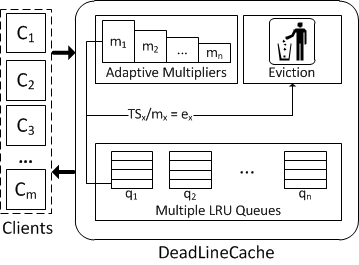
\includegraphics[scale=0.8]{img/DLC_arch.png}}
    \end{center}
  \end{figure}
\end{frame}

\begin{frame}
  \frametitle{DLC Interface Functions}
  \begin{figure}
    \begin{center}
      \centerline{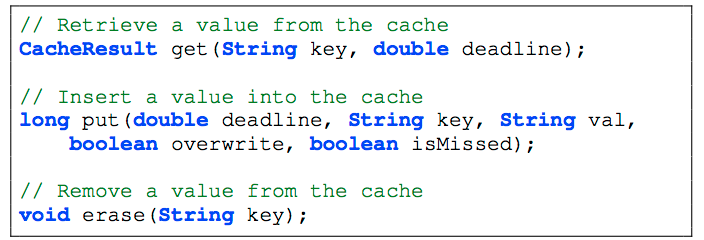
\includegraphics[scale=0.45]{img/DLC_interface.png}}
    \end{center}
  \end{figure}
\end{frame}

\begin{frame}
\frametitle{DLC - Adaptive Caching}
\begin{itemize}
\item DLC incorporates the cost of deadline misses
into its eviction policy by applying a queue specific
multiplier $\frac{1}{m_i}$ to the time difference between the current time
and the last access time of the item.
This difference is used to create a Modified Recency Value (MRV) for each eviction candidate.

\item The queue multipliers are adaptively computed using empirical measurements to reflect the likelihood
that a cache eviction would eventually lead to a deadline miss.
\end{itemize}


\end{frame}


\begin{frame}
\frametitle{DLC - Adaptive Caching Cont.}
\begin{itemize}
\item In our design, the multipliers are initialized to 1 and the system maintains the following invariant:
\begin{equation}
\label{eq:multiplier}
\sum\limits_{i=1}^n m_i = n
\end{equation}
\item Upon a receiving a \textit{put} request with a deadline within the range of queue $i$ and with
the deadline missed flag set to true, the multiplier $m_i$ is incremented by $\epsilon$
\item  To main the invariant in Equation 1, all of the queue multipliers are renormalized by
multiplying by $\frac{n}{n + \epsilon}$
\end{itemize}
\end{frame}


\begin{frame}
\frametitle{DLC - Advantages}
\begin{itemize}
\item Adaptiveness
\item Efficient computation
\item Deadline Aware
\item Tunable
\end{itemize}
\end{frame}


\begin{frame}
\frametitle{Deadline Scheduler (DLS) High-level Architecture}
  \begin{figure}
    \begin{center}
      \centerline{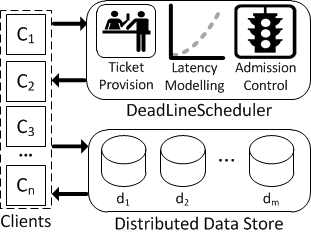
\includegraphics[scale=0.90]{img/DLS.png}}
    \end{center}
  \end{figure}
\end{frame}

\begin{frame}
\frametitle{DLS Interface Function}
  \begin{figure}
    \begin{center}
      \centerline{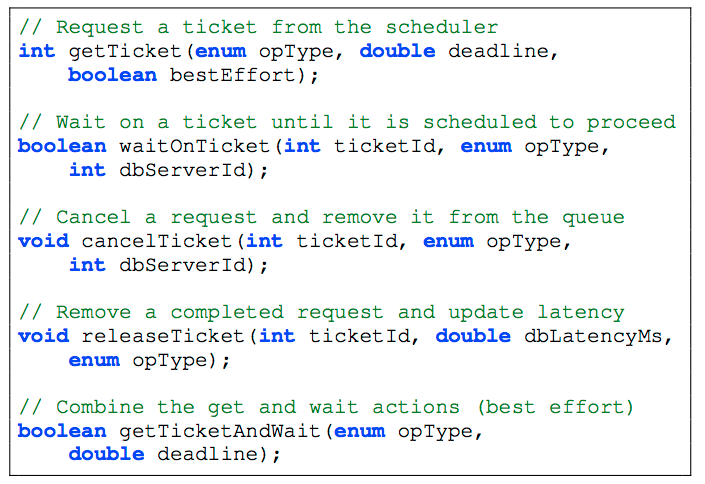
\includegraphics[scale=0.40]{img/DLS_interface.png}}
    \end{center}
  \end{figure}
\end{frame}

\begin{frame}
\frametitle{DLS - Ticket-Based Load-Balancing}
\begin{itemize}
\item Most cloud storage systems perform data replication
to provide fault tolerance, increase availability and improve read performance.
\item MicroFuge utilizes replications to improve read performance.
\item Randomly select two servers to request tickets.
\item Pick the the the server who claims to be able to satisfy the request deadline.
\end{itemize}
\end{frame}

\begin{frame}
\frametitle{DLS - Scheduling Algorithm}
\begin{itemize}
\item Uses an efficient variant of earliest deadline first (EDF) scheduling to determine the ordering
of pending requests.
\item EDF is known to be optimal for single-resource scheduling with preemption,
but EDF's scheduling can lead to additional deadline violations if the system is overloaded.
\item The DLS variant of EDF examines the response time performance model
of the storage server in order to determine whether a pending request should be scheduled
using its specified deadline, or rescheduled using a much larger artificial deadline in the case
where a deadline violation is inevitable.
\item To prevent starvation, DLS only allows a request to be rescheduled once.
\end{itemize}
\end{frame}

\begin{frame}
\frametitle{DLS - Scheduling Algorithm Cont.}
\begin{itemize}
\item The response time performance model uses request latencies from a past window of requests to
generate a latency distribution.
% TODO: Make this better
\item The system parameter $\alpha$ - we use the $\alpha$-percentile request
latency in the previous window to predict the latency for all the requests in the pending queue.
\item If inserting an item by the EDF algorithm will make any request violate its deadline, we can not meet
the new request's deadline.
\end{itemize}
\end{frame}

\begin{frame}
\frametitle{DLS - Optional Admission Control}
\begin{itemize}
\item Can be turned on or off.
\item If we can not meet a request's deadline, we reject it immediately.
\item Allows clients to quickly react.
\item The system parameter $\beta$
\begin{itemize}
\item Higher $\beta$ value will lead to fewer deadline miss but higher rejection rate.
\item Lower $\beta$ value will lead to the opposite effect.
\end{itemize}
\end{itemize}
\end{frame}

\begin{frame}
\frametitle{Full MicroFuge - MicroFuge Protocol}
Simple and elegant interface to the clients.
  \begin{figure}
    \begin{center}
      \centerline{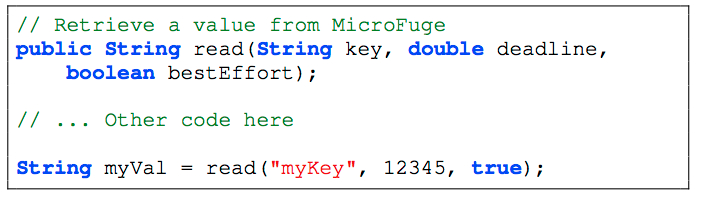
\includegraphics[scale=0.50]{img/MicroFuge_protocol.png}}
    \end{center}
  \end{figure}
\end{frame}

\begin{frame}
\frametitle{Full MicroFuge - An example}
Sample timeline for a read request from a client.
For this request, the requested item is not contained in the cache
and both schedulers accept the ensuing ticket requests.
  \begin{figure}
    \begin{center}
      \centerline{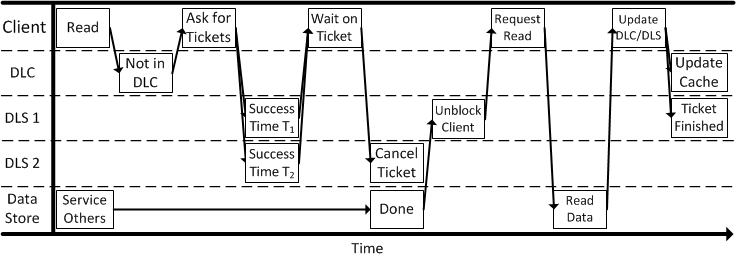
\includegraphics[scale=0.60]{img/RequestTimelineHorizontal.png}}
    \end{center}
  \end{figure}
\end{frame}


\begin{frame}
\frametitle{Experimental Setup - The Cluster}
\begin{itemize}
\item Twenty-node test cluster on Amazon Web Services
\item Each cluster node is an m1.medium EC2 instance
\begin{itemize}
\item 2 ECU
\item 3.7 GB memory - Manually reduced to 2 GB
\item 410 GB storage
\item Moderate Network Performance
\end{itemize}
\item Four Servers and Sixteen Clients.
\item YCSB benchmarks running on Clients.
\item MicroFuge or Memcached running on Servers.
\end{itemize}
\end{frame}


\begin{frame}
\frametitle{Experimental Setup - The Workload}
\begin{itemize}
\item Data set - key-value store with 80 million records, 86.4 GB in size.
\item Total cache capacity of our system is 19.2 GB - about 1/5th the size of the data set.
\item YCSB generated workloads. Slightly modified version.
\item Modified YCSB generates requests with various deadlines.
\item Particular key will always have the same deadline.
\item Deadlines fall into 3 ranges or buckets of deadlines:
[10=30) milliseconds, [30-100) milliseconds and [100-1000] milliseconds
\item Ranges' distribution ratio is 2:3:5 respectively.
\end{itemize}
\end{frame}



\begin{frame}
\frametitle{Experimental Results - Deadline Miss 1}
\begin{figure}[t]
\begin{center}
\centerline{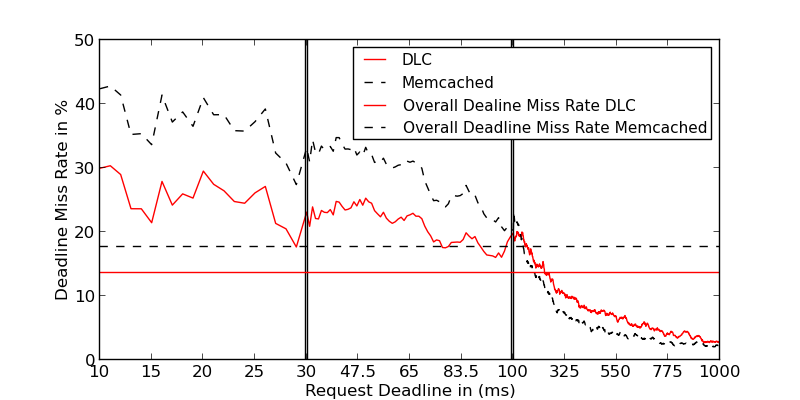
\includegraphics[scale=0.5]{img/EC2/EC2_CS_MM/miss_48.png}}
\caption{Deadline miss rate for 192 concurrent clients with DLC and Memcached.}
\label{fig:miss_192_cs_mm}
\end{center}
\end{figure}
\end{frame}



\begin{frame}
\frametitle{Experimental Results - Deadline Miss 2}
\begin{figure}[t]
\begin{center}
\centerline{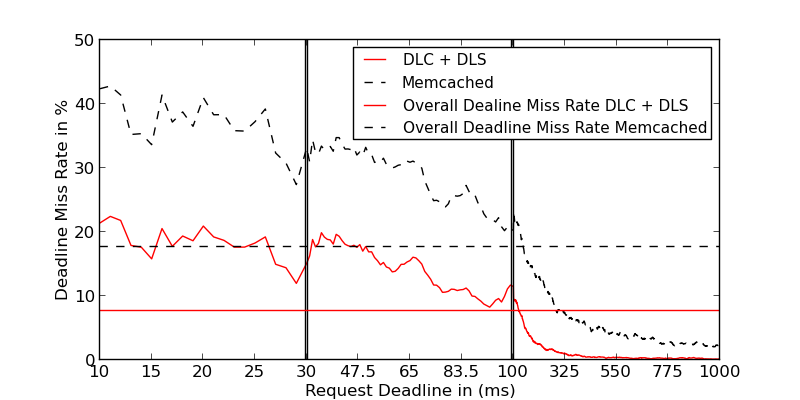
\includegraphics[scale=0.5]{img/EC2/EC2_SH_MM/miss_48.png}}
\caption{Deadline miss rate for 192 concurrent clients with DLC + DLS and Memcached.}
\label{fig:miss_192_sh_mm}
\end{center}
\end{figure}
\end{frame}

\begin{frame}
\frametitle{Experimental Results - Deadline Miss 3}
\begin{figure}[t]
\begin{center}
\centerline{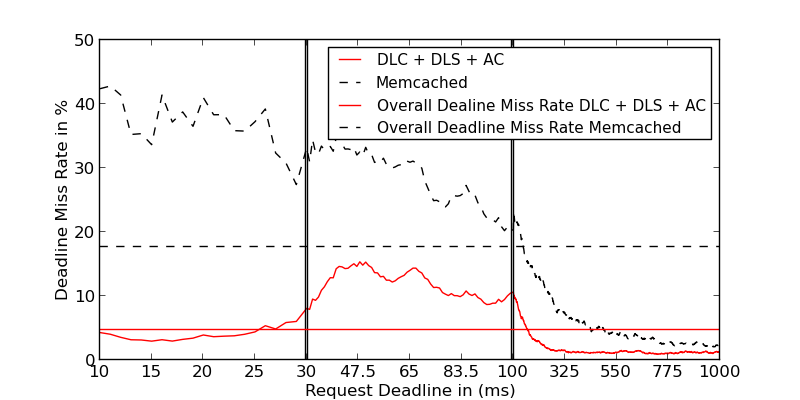
\includegraphics[scale=0.5]{img/EC2/EC2_AC_MM/miss_48.png}}
\caption{Deadline miss rate for 192 concurrent clients with DLC + DLS + AC and Memcached.}
\label{fig:miss_192_ac_mm}
\end{center}
\end{figure}
\end{frame}

\begin{frame}
\frametitle{Experimental Results - Caching 1}
\begin{figure}[t]
\begin{center}
\centerline{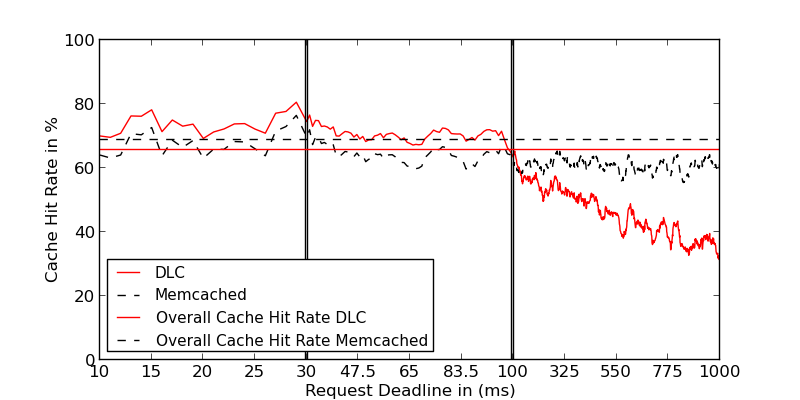
\includegraphics[scale=0.5]{img/EC2/EC2_CS_MM/cache_48.png}}
\caption{Cache hit rate for 192 concurrent clients with DLC and Memcached.}
\label{fig:cache_192_cs_mm}
\end{center}
\end{figure}
\end{frame}

\begin{frame}
\frametitle{Experimental Results - Caching 2}
\begin{figure}[t]
\begin{center}
\centerline{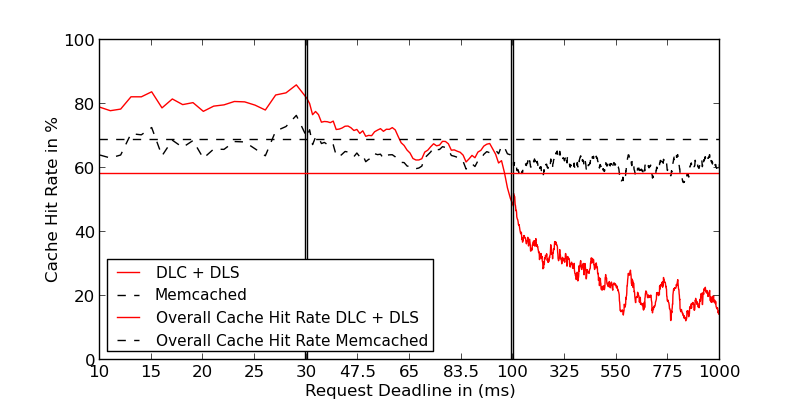
\includegraphics[scale=0.5]{img/EC2/EC2_SH_MM/cache_48.png}}
\caption{Cache hit rate for 192 concurrent clients with DLC + DLS and Memcached.}
\label{fig:cache_192_sh_mm}
\end{center}
\end{figure}
\end{frame}



\begin{frame}
\frametitle{Experimental Results - Tunable Admission Control}
\begin{figure}[t]
\begin{center}
\centerline{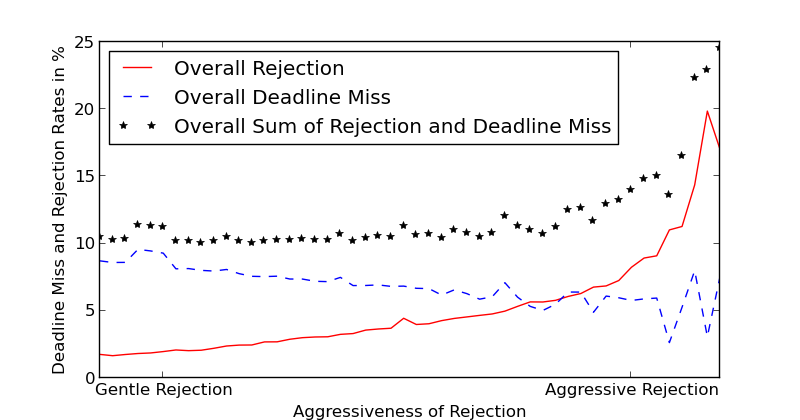
\includegraphics[scale=0.5]{img/EC2/Varying_ac/varying_acPerc_192.png}}
\caption{Deadline miss rate vs. rejection with respect to aggressiveness of rejection policy for 192 clients.}
\label{fig:deadline_miss_vs_rejection}
\end{center}
\end{figure}
\end{frame}


\begin{frame}
\frametitle{Experimental Results - Overall Miss Rates}
\begin{figure}[t]
\begin{center}
\centerline{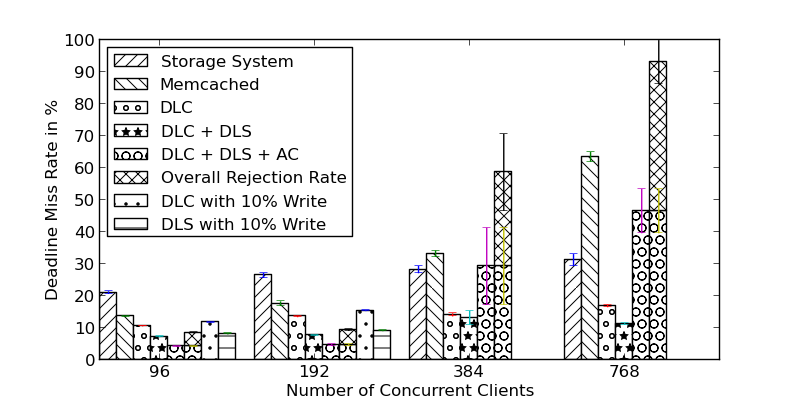
\includegraphics[scale=0.5]{img/EC2/EC2_BAR/miss_bar.png}}
\caption{Overall deadline miss rate with various numbers of concurrent clients (for 10\% write workloads
only results for 96 and 192 clients were generated).}
\label{fig:bar_miss}
\end{center}
\end{figure}
\end{frame}

\begin{frame}
\frametitle{Experimental Results - Overall Cache Hit Rates}
\begin{figure}[t]
\begin{center}
\centerline{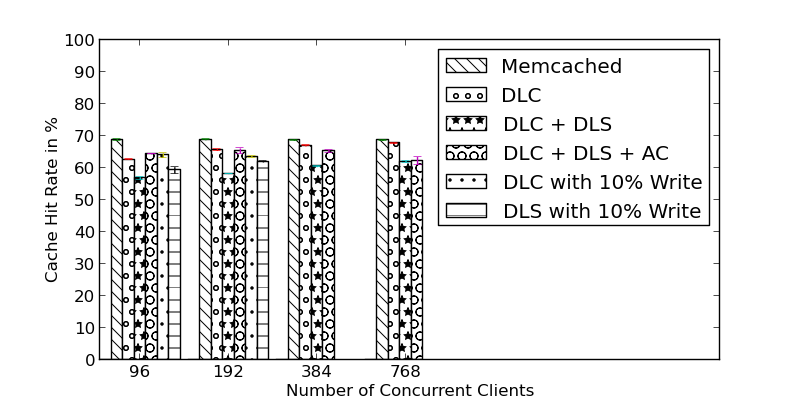
\includegraphics[scale=0.5]{img/EC2/EC2_BAR/cache_bar.png}}
\caption{Overall cache hit rates with various numbers of concurrent clients (for 10\% write workloads
only results for 96 and 192 clients were generated).}
\label{fig:bar_cache}
\end{center}
\end{figure}
\end{frame}

\section*{Conclusion and Future Work}
\begin{frame}
\frametitle{Conclusion and Future Work}
\begin{itemize}
\item MicroFuge - a new middleware layer that provides distributed scheduling and caching services to cloud storage systems.
\item Deadline-aware - reduce deadline miss rate from 20\% to less than 5\%.
\item Easy to layer on top of existing storage systems.
\item Explore fairness in context of deadline-aware.
\item Win the marketing campaign over Memcached and make it popular.
\end{itemize}
\end{frame}



\begin{frame}
\frametitle{References}
\begin{itemize}
\item Akshay K. Singh, Xu Cui, Benjamin Cassell, Bernard Wong, Khuzaima Daudjee, MicroFuge: A Middleware Approach to Providing Performance Isolation in Cloud Storage Systems.
\end{itemize}
\end{frame}

\end{document}
